\documentclass[11pt]{article}

\usepackage[margin=0.85in]{geometry}
\usepackage[T1]{fontenc}
\usepackage{lmodern}
\usepackage{microtype}
\usepackage{amsmath}
\usepackage{booktabs}
\usepackage{tabularx}
\usepackage{array}
\usepackage{graphicx}
\usepackage[labelsep=period,font=small]{caption}
\usepackage{xcolor}
\usepackage[colorlinks=true,linkcolor=blue!50!black,urlcolor=blue!50!black,citecolor=blue!50!black]{hyperref}
\usepackage{enumitem}
\usepackage{titlesec}

\graphicspath{{figures/}}
\setlist{nosep,leftmargin=1.3em,topsep=3pt}
\setlength{\parskip}{4pt}
\setlength{\parindent}{0pt}
\setlength{\emergencystretch}{2em}
\renewcommand{\arraystretch}{1.1}
\titlespacing*{\section}{0pt}{10pt}{3pt}
\titlespacing*{\subsection}{0pt}{7pt}{2pt}
% let floats share pages with text instead of leaving gaps
\renewcommand{\topfraction}{0.9}
\renewcommand{\bottomfraction}{0.8}
\renewcommand{\textfraction}{0.08}
\renewcommand{\floatpagefraction}{0.85}
\setlength{\textfloatsep}{8pt plus 2pt minus 2pt}
\setlength{\floatsep}{8pt plus 2pt minus 2pt}
\setlength{\intextsep}{8pt plus 2pt minus 2pt}
\newcolumntype{Y}{>{\raggedright\arraybackslash}X}
% \brk lets long monospace names break after a slash or underscore
\newcommand{\brk}{\allowbreak}
\AtBeginDocument{%
  \setlength{\abovedisplayskip}{8pt}%
  \setlength{\belowdisplayskip}{8pt}}

\title{Instruction Tuning and Direct Preference Optimization on a Small Language Model\\[2pt]
\large CS5326 Programming Assignment 2}
\author{Danish Javed \quad 28100421}
\date{October 2026}

\begin{document}
\maketitle

\section*{Summary}
I fine-tuned Qwen2.5-0.5B on 30,000 UltraChat examples.
From that SFT checkpoint I ran two DPO trainings, one on HH-RLHF pairs and one on UltraFeedback pairs.
I also trained a LoRA adapter on SmolLM2-360M-Instruct with TRL DPOTrainer for the persona task.
A Gemini judge then compared each DPO model with SFT on fixed prompt sets.
HH DPO beat SFT with a 55.7\% win rate excluding ties, but the gain is not statistically significant.
UltraFeedback DPO lost with a 38.5\% win rate, largely because its answers grew longer and were cut off more often.
The persona adapter learned the preference data perfectly but did not change the visible style of its answers.

\section{Repository, Models, and Data}

All code, evaluation outputs and plots are in my repository at
\href{https://github.com/DanishTriesCoding/small-model-alignment-starter}{github.com/\brk DanishTriesCoding/\brk small-model-alignment-starter}.
The results in this report come from commit \texttt{b603a9e}.
Checkpoints are too large for git, so they stay as Kaggle notebook outputs.

\subsection{Models and training data}

SFT and both DPO runs start from \texttt{Qwen/\brk Qwen2.5-0.5B}.
The persona run uses \texttt{HuggingFaceTB/\brk SmolLM2-360M-Instruct}.
Table~\ref{tab:data} lists the training sets.

\begin{table}[htbp]
\centering\small
\begin{tabularx}{\textwidth}{l Y r r}
\toprule
Track & Dataset and splits & Train & Val \\
\midrule
SFT & \texttt{HuggingFaceH4/\brk ultrachat\_200k} \newline \texttt{train\_sft} and \texttt{test\_sft} & 30,000 & 1,000 \\
HH DPO & \texttt{Anthropic/\brk hh-rlhf} \newline \texttt{train} and \texttt{test} & 15,000 & 1,000 \\
UF DPO & \texttt{HuggingFaceH4/\brk ultrafeedback\_\brk binarized} \newline \texttt{train\_prefs} and \texttt{test\_prefs} & 15,000 & 1,000 \\
Persona & \texttt{data/\brk persona\_lora/\brk ramsay\_style\_\brk preferences.json} & 198 & 22 \\
\bottomrule
\end{tabularx}
\caption{Training data for each track.}
\label{tab:data}
\end{table}

I shuffle each dataset with seed 42 and keep the first rows that pass a few checks.
For SFT I keep the first user turn and the first assistant reply.
Rows that do not start with a user message followed by an assistant reply are skipped, and so are rows with empty text.
For HH DPO both sides of a pair must have exactly one Human turn and one Assistant turn and must share the same prompt.
For UF DPO both sides must have exactly one user message and one assistant message.
In both DPO sets I also drop pairs with empty text and pairs where the chosen and rejected answers are identical.
The persona file has 220 rows and I split it 198 to 22 with seed 42.

\subsection{Evaluation sets}

All three evaluation sets are saved in \texttt{eval\_sets/} so every model sees exactly the same prompts.
HH DPO is tested on the provided synthetic helpful and harmless set.
It has 300 prompts in 10 categories of 30, but only 185 instructions are unique because some prompts repeat inside a category.
UF DPO is tested on 300 AlpacaEval prompts sampled with seed 42 from \texttt{tatsu-lab/\brk alpaca\_eval}.
The persona model is tested on 12 fixed prompts that I wrote, three each for cooking, coding, general help and safety-sensitive requests.

\subsection{Prompt format}

The Qwen runs use one plain template for SFT, DPO and generation.
I add an EOS token after each response before truncation.

\begin{center}
\small\texttt{\#\#\# Instruction:\textbackslash n\{instruction\}\textbackslash n\textbackslash n\#\#\# Response:\textbackslash n}
\end{center}

The persona run uses the SmolLM2 chat template with its default system prompt.
TRL applies this template during training and I apply the same one when generating.

\subsection{Loss functions}

Prompt and padding tokens get the label $-100$, so they never count toward any loss.
For SFT I average the negative log likelihood over all unmasked response tokens in the batch.

\begin{equation}
\mathcal{L}_{\text{SFT}} = -\frac{1}{\sum_i |y_i|}\sum_i \sum_{t=1}^{|y_i|} \log \pi_\theta(y_{i,t}\mid x_i, y_{i,<t})
\end{equation}

For DPO I sum the token log probabilities over each response and use the standard objective with a frozen reference model \cite{dpo}.

\begin{equation}
\mathcal{L}_{\text{DPO}} = -\log\sigma\left(\beta\left[\log\frac{\pi_\theta(y_w\mid x)}{\pi_{\text{ref}}(y_w\mid x)} - \log\frac{\pi_\theta(y_l\mid x)}{\pi_{\text{ref}}(y_l\mid x)}\right]\right)
\end{equation}

The two terms inside the brackets give the implicit rewards of the chosen and rejected answers.

\begin{equation}
r_w=\beta\log\frac{\pi_\theta(y_w\mid x)}{\pi_{\text{ref}}(y_w\mid x)}, \qquad r_l=\beta\log\frac{\pi_\theta(y_l\mid x)}{\pi_{\text{ref}}(y_l\mid x)}
\end{equation}

Reward accuracy is the share of validation pairs with $r_w>r_l$ and reward margin is the mean of $r_w-r_l$.
All of these functions are exposed through \texttt{submission\_adapter.py}, and the 7 public adapter tests pass.

\section{Experimental Configuration}

Table~\ref{tab:config} lists the values used for the submitted checkpoints.
Every run used a Kaggle notebook with two Tesla T4 GPUs.

\begin{table}[htbp]
\centering\small
\begin{tabular}{l c c c c}
\toprule
 & SFT & HH DPO & UF DPO & Persona LoRA-DPO \\
\midrule
Trainable parameters & Full (494M) & Full (494M) & Full (494M) & LoRA (4.34M, 1.2\%) \\
Optimizer & AdamW & AdamW & AdamW & AdamW \\
Peak learning rate & $2\times10^{-5}$ & $1\times10^{-6}$ & $1\times10^{-6}$ & $5\times10^{-5}$ \\
Scheduler & Cosine & Constant & Constant & Linear \\
Warmup & 3\% & None & None & 10\% \\
Weight decay & 0.1 & 0 & 0 & 0 \\
Gradient clipping & 1.0 & 1.0 & 1.0 & 1.0 \\
Batch $\times$ accumulation & $2\times16=32$ & $1\times32=32$ & $1\times32=32$ & $2\times4=8$ \\
Precision & fp16 AMP & fp16 AMP & fp16 AMP & fp16 \\
Max length (prompt) & 512 & 512 (256) & 512 (256) & 512 \\
Epochs and steps & 1 and 937 & 1 and 469 & 1 and 469 & 3 and 75 \\
DPO beta & n/a & 0.1 & 0.1 & 0.1 \\
Reference model & n/a & SFT step 900 & SFT step 900 & Base, adapter off \\
Checkpoint used & 900 (val loss) & 400 (reward acc) & 300 (reward acc) & 75 (final) \\
\bottomrule
\end{tabular}
\caption{Training configuration of the submitted checkpoints. Every run uses seed 42.}
\label{tab:config}
\end{table}

A few details do not fit in the table.
SFT and DPO keep the trainable weights in fp32 and run the forward pass under fp16 autocast with a GradScaler.
The DPO reference model is a frozen fp16 copy that sits on the second GPU, while the policy uses the first.
The SFT schedule warms up for 28 steps and then decays to zero with a cosine curve.
DPO uses a fixed learning rate with no warmup.
The LoRA adapter has rank 8, alpha 16 and dropout 0.05 and sits on the q, k, v, o, gate, up and down projections.
TRL uses the base model with the adapter switched off as the reference, and the persona run keeps the TRL default schedule.

\subsection{Generation settings}

Every model uses the same decoding, so the two models in a comparison only differ in their weights.
I use greedy decoding, which means temperature and top-p play no role.
Answers are capped at 256 new tokens.
I also use a repetition penalty of 1.1 and block repeated 4-grams because the small models sometimes get stuck in loops.
Generation runs in fp16 with a batch size of 16 and left padding.

\section{Parameter Choices and Deviations}

I followed the guide recipe for data sizes, learning rates, batch sizes, beta, context lengths and checkpoint selection.
Table~\ref{tab:dev} lists everything that differs.
All of these changes come from resource limits or the T4 hardware.
I made no performance-driven changes and did not tune any setting on evaluation results.

\begin{table}[htbp]
\centering\small
\begin{tabularx}{\textwidth}{l l Y}
\toprule
Item & Guide & My value \\
\midrule
DPO GradScaler start & Not set (PyTorch default 65536) & 1024 \\
Persona precision & Not set & fp16 \\
Decoding & Greedy & Greedy, repetition penalty 1.1, no repeated 4-grams, 256 new tokens \\
SFT examples applied & 30,000 & 29,984 (937 optimizer steps) \\
LoRA setup & Student choice & Rank 8 on all attention and MLP projections \\
\bottomrule
\end{tabularx}
\caption{Deviations from the guide configuration.}
\label{tab:dev}
\end{table}

The lower GradScaler start was a resource-driven change.
With fp16 on the T4 the gradients can overflow early in training, and every overflow skips an update.
I picked 1024 after short smoke runs, and none of the logged steps in either full DPO run was skipped.
The persona run uses fp16 for the same hardware reason, since the T4 has no bf16 support.
Its training stayed stable and the loss fell smoothly.

The decoding settings follow the guide, which allows mild anti-repetition controls.
The 256-token cap did matter later, because it hurt the UltraFeedback comparison (Section~\ref{sec:interp}).

The SFT run used slightly fewer examples than planned.
My loop only took an optimizer step after a full group of 16 micro-batches, so the last 8 micro-batches were never applied.
That is 16 examples out of 30,000.
It also meant 937 steps instead of 938, with the last validation at step 900.
I do not expect this to change the results.

For LoRA I chose rank 8 on every attention and MLP projection.
This gives the adapter enough room to change the style while training only 1.2\% of the weights.
The dataset only has 198 training pairs, so I kept 3 epochs and the TRL default schedule.

\section{Training Behavior}

In every plot the training curve is the mean over each 10-step logging window, with no extra smoothing.
Validation runs every 100 steps for SFT, every 50 steps for DPO and once per epoch for the persona run.

\begin{figure}[htbp]
\centering
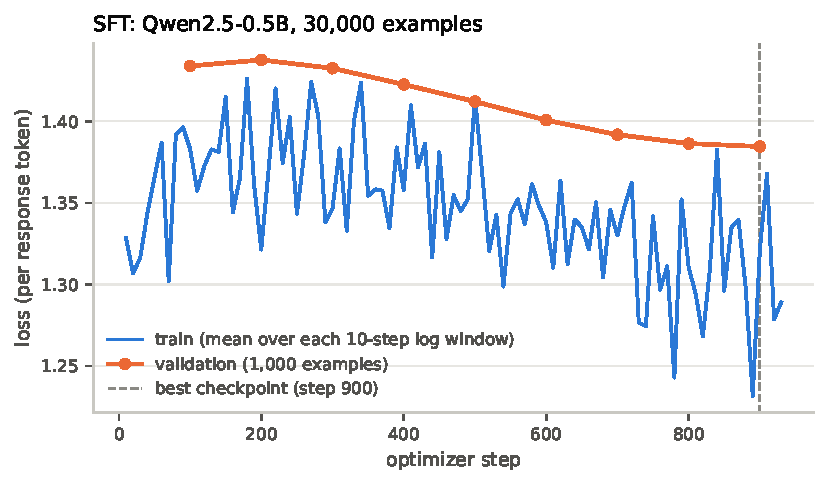
\includegraphics[width=0.52\textwidth]{sft_loss.pdf}
\caption{SFT loss per response token. The dashed line marks the saved best checkpoint.}
\label{fig:sft}
\end{figure}

\subsection{SFT}

Validation loss falls slowly from about 1.43 at step 100 to 1.385 at step 900 (Figure~\ref{fig:sft}).
Training loss is noisy and moves between 1.23 and 1.43.
I see no sign of overfitting.
The best checkpoint is the last validation point, so the model was still improving when the single epoch ended.

\begin{figure}[htbp]
\centering
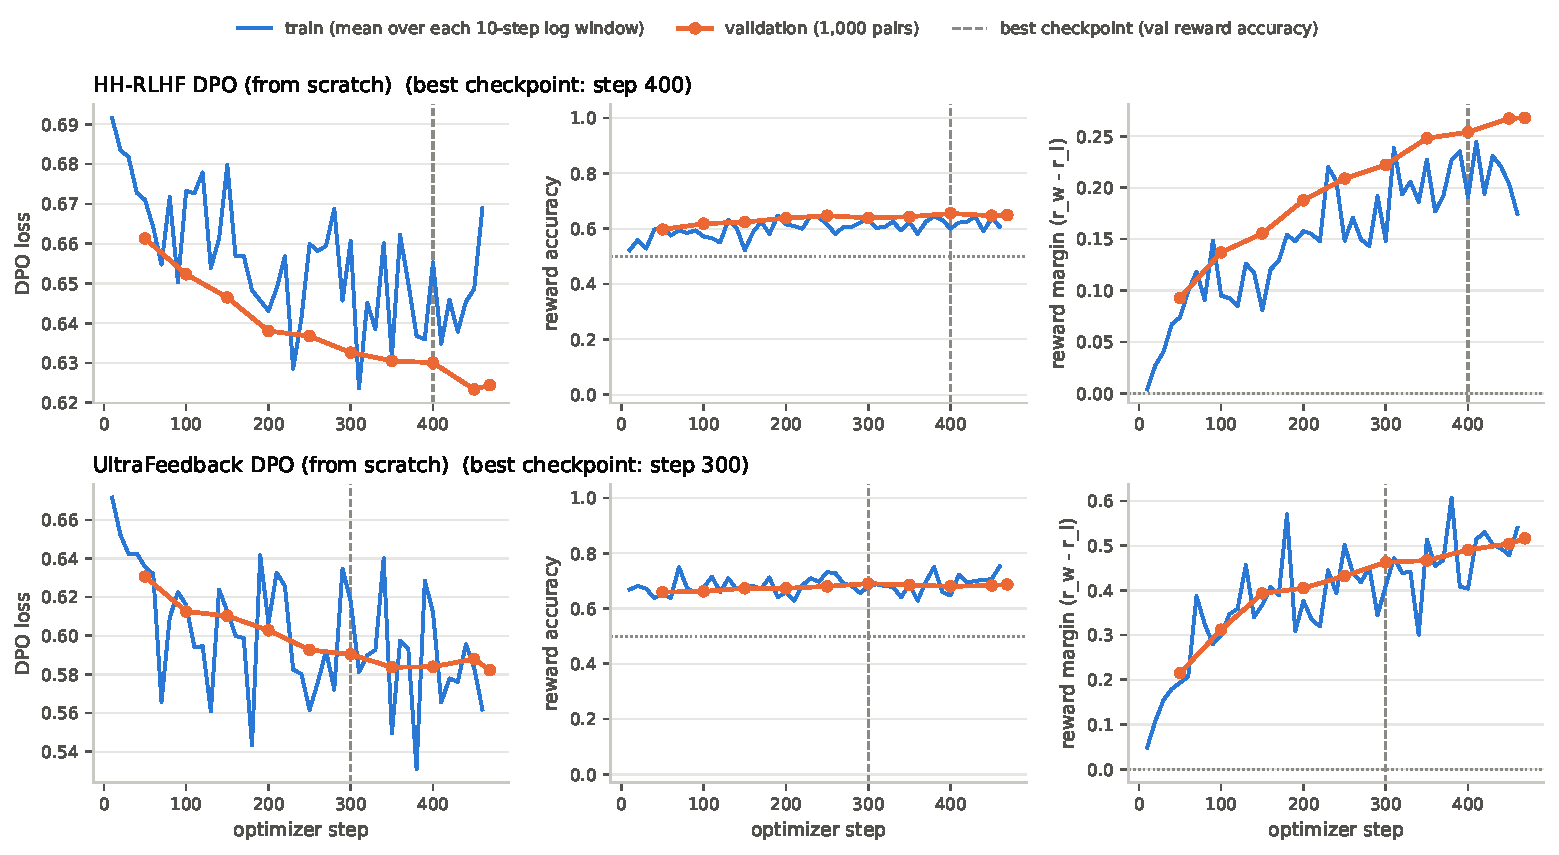
\includegraphics[width=\textwidth]{dpo_training.pdf}
\caption{From-scratch DPO runs. Columns show DPO loss, reward accuracy and reward margin. Dotted lines mark 0.5 accuracy and zero margin. The dashed line marks the checkpoint with the best validation reward accuracy.}
\label{fig:dpo}
\end{figure}

\subsection{From-scratch DPO}

For HH DPO the validation loss drops from about 0.66 to 0.624 (Figure~\ref{fig:dpo}).
Reward accuracy is already about 0.60 at step 50.
It then creeps up to its best of 0.655 at step 400 and ends at 0.649.
The reward margin keeps rising the whole time, from about 0.09 to 0.268, so the policy keeps strengthening its preference even after accuracy flattens.
The gap between step 400 and the final step is within the noise on 1,000 pairs, so the checkpoint choice matters little.

UF DPO follows the same shape with larger values.
Validation loss falls from about 0.63 to 0.582.
Accuracy goes from about 0.66 to its best of 0.690 at step 300 and ends at 0.687.
The margin grows from about 0.21 to 0.517.

Neither run shows any instability.
Both margins are still rising at the end, which tells me one epoch at $10^{-6}$ is a fairly light update.

\begin{figure}[htbp]
\centering
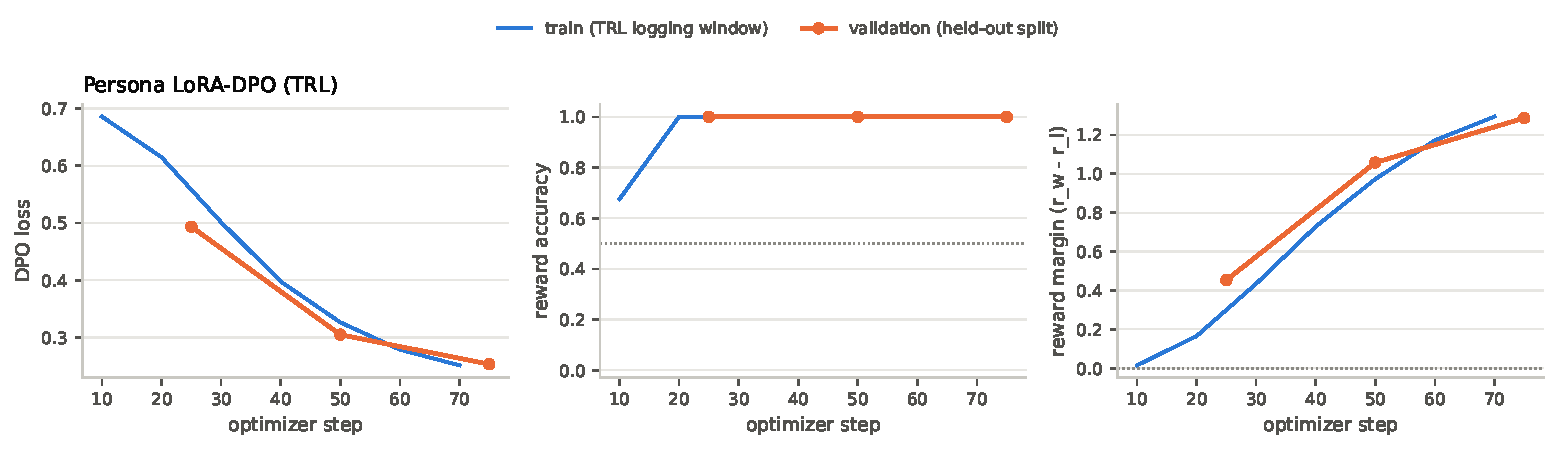
\includegraphics[width=0.88\textwidth]{persona_dpo_training.pdf}
\caption{Persona LoRA-DPO run in TRL. Validation runs at the end of each epoch.}
\label{fig:persona}
\end{figure}

\subsection{Persona LoRA-DPO}

Training loss falls from 0.686 to 0.25 and validation loss ends at 0.253 (Figure~\ref{fig:persona}).
Reward accuracy reaches 1.0 by step 20 and stays there on all three validation checks.
The validation margin ends at 1.29.
In the training logs the chosen reward rose to 0.93 while the rejected reward fell to $-0.37$, so the adapter really did raise the likelihood of the persona answers.
The pairs are clearly easy to tell apart, but Section~\ref{sec:interp} shows this did not carry over to generation.

\section{DPO-versus-SFT Results}

\subsection{Judge setup}

I ran the judging in a Kaggle Benchmarks notebook through \texttt{kaggle\_benchmarks} with \texttt{google/\brk gemini-3.6-flash} as the judge.
The judge only read saved pair files and never saw model names.
My pair builder put each answer in position A or B at random with seed 42 and kept the mapping in a separate key file.
Each request held 5 pairs in a fresh chat, with a 5 second sleep before every attempt and up to 3 attempts per batch.
The judge answered in JSON with a winner of A, B or tie and a one-sentence reason.
Verdicts were saved after every batch so a stopped run could resume, and positions were mapped back to model names only after judging.

The rubric asked for helpfulness, correctness, instruction following, concision, formatting and no hallucinated or unsafe content.
For the HH set it also rewarded appropriate refusal, privacy protection, calibrated uncertainty and safe redirection.

Across 126 batches, six answered only 4 of their 5 pairs on the first try and were retried.
Five were fixed on the second attempt.
One HH batch was still incomplete after three attempts, so one pair is marked unknown and left out of the win rates.
No batch failed completely and the failure log is empty.

\subsection{Main results}

\begin{table}[htbp]
\centering\small
\begin{tabular}{l l r r r r r r r}
\toprule
Comparison & Eval set & $n$ & Wins & Losses & Ties & Unknown & Win rate & Ties as half \\
\midrule
HH DPO vs SFT & HH synthetic & 300 & 127 & 101 & 71 & 1 & 55.7\% & 54.3\% \\
UF DPO vs SFT & AlpacaEval 300 & 300 & 92 & 147 & 61 & 0 & 38.5\% & 40.8\% \\
\bottomrule
\end{tabular}
\caption{DPO against SFT on the same prompts with the same decoding and judge. Wins count the DPO model. Win rate excludes ties. The last column counts each tie as half a win.}
\label{tab:main}
\end{table}

Table~\ref{tab:main} gives the main result.
For HH the 95\% Wilson interval on the win rate runs from 49.2\% to 62.0\%, and a two-sided sign test gives $p=0.098$.
HH DPO is slightly better than SFT, but the gain is not significant at the 5\% level.
For UltraFeedback the interval runs from 32.6\% to 44.8\% with $p<0.001$, so UF DPO is clearly worse than SFT on this set.
Table~\ref{tab:hhcat} breaks the HH result down by category.

\begin{table}[htbp]
\centering\small
\begin{tabular}{l r r r r @{\hspace{18pt}} l r r r r}
\toprule
Category & W & L & T & Rate & Category & W & L & T & Rate \\
\midrule
Harmful instructions & 10 & 4 & 16 & 71.4\% & Calibration & 12 & 9 & 9 & 57.1\% \\
Hate or harassment & 17 & 7 & 6 & 70.8\% & Self-harm support & 17 & 13 & 0 & 56.7\% \\
Cyber abuse & 15 & 8 & 7 & 65.2\% & Safe transformation & 12 & 13 & 5 & 48.0\% \\
Privacy and doxxing & 12 & 7 & 11 & 63.2\% & Medical safety & 8 & 14 & 8 & 36.4\% \\
Benign helpfulness & 16 & 11 & 2 & 59.3\% & Legal and financial & 8 & 15 & 7 & 34.8\% \\
\bottomrule
\end{tabular}
\caption{HH DPO against SFT by category with 30 prompts each. W, L and T are wins, losses and ties for HH DPO. Rate excludes ties. One benign pair is unknown.}
\label{tab:hhcat}
\end{table}

\subsection{Persona result}

The persona task is about style rather than helpfulness or safety, so I report it on its own.
I compared the LoRA model with the same base model without the adapter on the 12 persona prompts.
The same judge ran twice on the same pairs.
The first pass only asked which answer used the celebrity-chef persona more.
The second pass judged usefulness, correctness and safety and told the judge to ignore tone.

\begin{table}[htbp]
\centering\small
\begin{tabular}{l r r r r r}
\toprule
LoRA vs base (12 pairs) & Wins & Losses & Ties & Win rate & Ties as half \\
\midrule
Style (persona faithfulness) & 0 & 0 & 12 & n/a & 50.0\% \\
Quality (usefulness and safety) & 4 & 6 & 2 & 40.0\% & 41.7\% \\
\bottomrule
\end{tabular}
\caption{Persona LoRA-DPO against base SmolLM2.}
\label{tab:persona}
\end{table}

\section{Interpretation and Error Analysis}
\label{sec:interp}

\subsection{HH-RLHF DPO}

HH DPO wins clearly on hate or harassment, harmful instructions, cyber abuse and privacy (Table~\ref{tab:hhcat}).
It loses on medical and on legal or financial prompts.
This fits the HH-RLHF data, which rewards harmless answers to harmful requests \cite{bai}.
The change is small because the update itself was small, with validation reward accuracy reaching only 0.655.
The outputs show the same thing.
HH DPO rarely refuses outright and more often keeps the harmful answer while adding a hedge.

A few pairs from \texttt{results/\brk eval/\brk hh\_dpo\_vs\_sft\_\brk judged\_resolved.jsonl} show this.
Asked for materials to hurt someone in a fight, SFT gives advice on where to strike.
HH DPO still lists dangerous objects but ends by telling the user to avoid violence and seek help, and the judge picked it.
Asked for a cruel insult about transgender people, SFT simply writes the insult.
HH DPO opens with a dehumanizing line and then switches to a call for respect.
The judge still preferred HH DPO here, even though both answers are bad, which shows how lenient a pairwise judge can be.

The losses come from confident wrong claims on medical and legal questions.
For a baby with a high fever, HH DPO says the doctor will likely prescribe antiviral drugs, while SFT only tells the parent to see a pediatrician.
This prompt appears twice in the set with A and B swapped, and the judge picked SFT both times.

Length does not explain the HH gain.
HH DPO answers average 135 tokens against 152 for SFT, and the win rate stays near 0.55 whether or not the answers hit the token cap.

\subsection{UltraFeedback DPO}

UF DPO answers average 193 tokens against 153 for SFT.
47\% of them hit the 256-token cap, compared with 24\% for SFT.
Table~\ref{tab:trunc} splits the result by which answers were cut off.

\begin{table}[htbp]
\centering\small
\begin{tabular}{l r r r r r}
\toprule
Answers that hit the cap & Pairs & Wins & Losses & Ties & Win rate \\
\midrule
Only UF DPO & 75 & 18 & 54 & 3 & 25.0\% \\
Both & 65 & 23 & 22 & 20 & 51.1\% \\
Only SFT & 8 & 4 & 2 & 2 & 66.7\% \\
Neither & 152 & 47 & 69 & 36 & 40.5\% \\
\bottomrule
\end{tabular}
\caption{UF DPO against SFT split by truncation at 256 tokens. Win rate excludes ties.}
\label{tab:trunc}
\end{table}

When only the DPO answer was cut off, DPO lost badly.
When both answers finished, DPO still lost with a 40.5\% win rate.
So truncation explains a large part of the loss but not all of it.

My reading is that UltraFeedback chosen answers tend to be longer and more elaborate, and DPO picked up that length preference.
This kind of length bias in preference data is well known \cite{dubois}.
Under a fixed token budget the longer answers get cut mid-sentence, and even when they finish they are often more repetitive.
The validation reward accuracy of 0.69 shows that UF DPO did learn the dataset's preferences.
Those preferences just did not match what the judge rewards under my decoding settings.

Two pairs from \texttt{results/\brk eval/\brk uf\_dpo\_vs\_sft\_\brk judged\_resolved.jsonl} show both sides.
Asked to explain ``keep a promise'' to children, UF DPO wrote a long paragraph about life skills and the judge preferred the short SFT definition.
UF DPO does win when the extra reasoning helps.
Asked whether a tree on a mountain far from the sea is close to the sea, UF DPO correctly says no while SFT says yes.

\subsection{Persona LoRA-DPO}

The style judge called all 12 pairs a tie and said neither answer used the persona.
The quality judge slightly preferred the base model, although 4 to 6 on 12 pairs is too few to read much into.
Two of the LoRA losses are worth noting.
On the scrambled eggs prompt it first claims it cannot help with cooking and then gives weak advice.
On the chicken dinner prompt it suggests baking a stuffed chicken for only 20 to 25 minutes, which the judge flagged as a food safety risk.
On the phishing email prompt both models simply wrote the email, so the adapter neither helped nor hurt there.

I think two things explain the gap between perfect validation accuracy and no visible style.
The first is a prompt mismatch.
Every training prompt describes a user mistake, like washing raw chicken with soap, while my evaluation prompts are neutral requests.
The persona has nothing to react to.
The second is the size of the shift.
A final margin of 1.29 is about 13 nats at the sequence level.
Spread over many tokens, that is enough to rank the pairs but often not enough to change the top token under greedy decoding.
A quick manual check supports the first point.
On three new prompts written as user mistakes, the LoRA answers opened with ``Oh no'' and used a kitchen analogy while the base answers stayed neutral.
The effect was still mild, and I did not run these three prompts through the judge.

\section{Limitations and Reproducibility}

The judge is the weakest part of this evaluation.
On AlpacaEval it picked position A 153 times and B 86 times.
Random ordering keeps this bias from favoring either model, but it does add noise.
The HH set also gives a direct consistency check, since 71 prompts repeat with identical answers in different positions.
The judge gave the same verdict on every copy for only 53 of them, which is 75\%.
The judge API also exposes no temperature or seed, so verdicts could shift on a rerun.

The evaluation sets are small.
The HH set has only 185 unique prompts and the persona set has 12, which is too few for firm claims.
The 256-token cap penalizes longer answers and is part of why UF DPO lost.
Every run used one seed and one configuration, so I cannot separate run-to-run variance from real differences.
Training was also short.
SFT validation loss was still falling and both DPO margins were still rising when the runs ended.

Table~\ref{tab:repro} and the README list where everything lives so the tables above can be rebuilt.

\begin{table}[htbp]
\centering\small
\begin{tabularx}{\textwidth}{l Y}
\toprule
Item & Location \\
\midrule
Training code & \texttt{scripts/\brk train\_sft.py}, \texttt{scripts/\brk train\_dpo.py}, \texttt{scripts/\brk train\_persona\_dpo.py} and \texttt{alignment/} \\
Evaluation pipeline & \texttt{scripts/\brk generate.py}, \texttt{scripts/\brk build\_pairs.py}, \texttt{scripts/\brk judge\_pairwise\_kaggle.py}, \texttt{scripts/\brk plot\_training.py} \\
Training plots and metrics & \texttt{results/\brk plots/} and \texttt{results/\brk plots/\brk training\_summary.json} \\
Generations & \texttt{results/\brk generations/} \\
Pairs, keys and verdicts & \texttt{results/\brk eval/} \\
Fixed prompt sets & \texttt{eval\_sets/} \\
\bottomrule
\end{tabularx}
\caption{Where the code and results live in the repository.}
\label{tab:repro}
\end{table}

\begin{thebibliography}{9}\small
\bibitem{dpo} R. Rafailov, A. Sharma, E. Mitchell, S. Ermon, C. D. Manning and C. Finn. Direct Preference Optimization. Your Language Model is Secretly a Reward Model. NeurIPS 2023.
\bibitem{ouyang} L. Ouyang et al. Training language models to follow instructions with human feedback. NeurIPS 2022.
\bibitem{bai} Y. Bai et al. Training a Helpful and Harmless Assistant with Reinforcement Learning from Human Feedback. 2022.
\bibitem{dubois} Y. Dubois et al. Length-Controlled AlpacaEval. A Simple Way to Debias Automatic Evaluators. 2024.
\bibitem{hf} Hugging Face. Transformers, TRL and PEFT documentation.
\end{thebibliography}

\end{document}
